\documentclass[a4paper, 11pt]{article}
\usepackage[utf8]{inputenc}
\usepackage[english]{babel}
\usepackage{geometry}
\usepackage{multirow}
\usepackage{longtable}
\usepackage[usenames,dvipsnames]{xcolor}
\bibliographystyle{apalike}
\usepackage{apalike}
\usepackage{mathtools}
\usepackage{graphicx}
\usepackage{amsmath}

\author{Ángela Miranda Segura}
\title{bla bla bla bla}
\begin{document}
\maketitle
\begin{minipage}{4cm}
	\textbf{Keywords:}
	Chlorophyll, function, photosynthesis.
\end{minipage}
\begin{minipage}{7cm}
	\begin{abstract}
		hola
	\end{abstract}
\end{minipage}


\twocolumn
\section{Introduction}
 	A leaf with 7 millon cells houses, each containin approximately 600 millon molecules of chlorophyll. These $10^18$ chlorophyll mole-cules, all of which are bound to proteins of photosynthetic membranes, harvest the sunlight. Approximately 250 to 300 of them transfer the absorbed light energy through neighbouting pigments to the "especial pair" chlorophylls in a reaction center. These special pair chlorophylls in photosystems I and II are the primary electron donors that drive the conversion of light into chemical energy to be conserved in NADPH2 and ATP \cite{VonWettstein1995}
 	

	Chlorophylls are esential molecules that are responsible for harvesting solar energy in photosynthetic antenna systemas, and for charge separation and electron transport within reaction centers. Chlorophyll metabolism is a highly coordinated process that is executed via a series of cooperative reactions catalyzed by numerous enzymes.\\
	
	\subsection{The chlorophyll metabolic\\ pathway and its regulation} 
	Chlorophyll biosynthesis can be classified into three distinct phases (Figure 1). The first phase encompasses the synthesis of chlo-rophyll a from glutamate. Figure 1 depicts the chlorophyll a biosynthetic pathway such that the order of enzymatic steps involving divinyl protochlorophyllide a, \\vinyl reductase, and protochlorophyllide oxidoreductase differs from that in previously proposed schematics describing this pathway. We made this revision on the basis of recent findings describing the substrate specificity of divinyl protochlorophyllide a vinyl reductase. The second phase includes the interconversion of chlorophyll a and chlo-rophyll b, and is also known as the chlorophyll cycle \cite{Rudiger2002}. In this cycle, the in vivo substrate of chlorophyllide a oxygenase (CAO) remains unidentified, although in vitro experiments have shown that chlorophyllide a, rather than chlorophyll a, is a substrate of CAO \cite{Oster2000}. The third and final phase of chlorophyll metabolism involves the degradation of chlorophyll a \cite{Takamiya2000}. This degradation pathway has been traced from chlorophyll a through to the non-fluorescent chlorophyll catabolite (NCC). Clarification is still necessary, however, to determine whether NCC is further degraded to monopyrroles or other smaller molecules. A further question remains as to whether degraded chlorophyll is recycled as a nitrogen resource for building other macromolecules. Although most of the genes that encode the enzymes involved in chlorophyll metabolism have been identified, those encoding some key enzymes such as Mg-dechelatase are still to be identified \cite{Tanaka2006}
	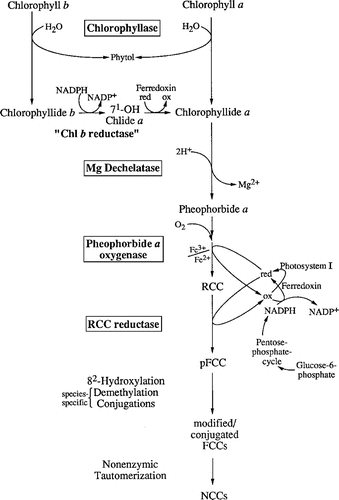
\includegraphics{figura2}
	
\section{State of art}
	Results of recent studies have better defined the chlorophyll metabolic pathway,\\ specifically by identifying the majority of the genes that are involved in the process. These recent advances have enabled significant progress toward understanding the me-chanisms that regulate chlorophyll meta-bolism. Regulation of the levels of chlorophyll and its derivatives is extremely important because these molecules are strong photosensitizers; that is, when present in excess, they will generate reactive oxygen species (ROS). ROS, in turn, promote\\ growth retardation or cell death. Therefore, to maintain healthy growth, plants must finely control the entire chlorophyll metabolic process.\\
	
	Additional studies have revealed preliminary information about the mechanisms that govern the trafficking of chlorophyll metabolic intermediates in plants. This level of control is especially important because, in response to cellular demand, plants produce various tetrapyrrole molecules, such as heme, siroheme and phytochromobilin, that are employed further in a variety of biochemical processes. Significant progress has also been made toward elucidating the linkages between chlorophyll metabolism and other cellular processes, including leaf senescence, programmed cell death, and plastid signaling. Although the molecular mechanisms that underlie these linkages remain elusive, these initial findings have motivated us to re-examine the physiological implications of chlorophyll metabolism \cite{Tanaka2006}

\section{Materials and methods}
	It has been studied the absorption of light by chlorophyl solutions using different methods which provide different results due to artifacts and teh susbtantial effect of solvent on the coefficinents. \\
	
	In Table 1, columns 2 and 3, are given the k values for the same preparation of chlotophylls a and b in aqueous acetone (20ml of distilled water per 80ml of redistilled anhydrous C.P. acetone). To bring the chlorophyll into solution, 2ml of acetone were used, then 0.5ml of water. The sample was the made to volumen. In column 7 is given the absorption of an Avena extract in this solvent \cite{Mackinney}.
	
	\restoregeometry
	\begin{longtable}{|c|c|c|c|c|c|c|}
		\hline
		\multirow{2}{*}{wavelength} & 
		\multicolumn{2}{c}{chlorophyll} & 
		\multicolumn{3}{c}{calculated contribution} & 
		\multirow{2}{*}{avena experimental kc} \\
		& $k_a^*$ & $k_b$ & $k_aC_a$ & $k_bC_b$ & Combined & \\ \hline
		6800 & 11.49 &&0.046 &&&0.049 \\
		6700 & 56.75 & 3.39 & 0.237 & 0.005 & 0.242 & 0.231\\
		6650 & 80.91 & 6.55 & 0.324 & 0.009 & 0.333 & 0.330\\
		6630 & 82.04 & 9.27 & 0.328 & 0.013 & 0.341 & 0.341\\
		6600 & 76.03 & 14.69 & 0.304 & 0.021 & 0.325 & 0.331\\
		6500 & 28.51 & 40.74 & 0.114 & 0.057 & 0.171 &0.177\\
		6450 & 16.75 & 45.60 & 0.068 & 0.064 & 0.132 & 0.131\\
		6400 & 12.39 & 34.51 &0.05 & 0.048 & 0.098 & 0.095\\
		6350 & 11.62 & 20.32 & 0.046 & 0.028 & 0.074 & 0.074\\
		6300 & 13.15 & 12.70 & 0.052 & 0.018 & 0.07 &0.068\\
		6200 & 16.37 & 9.06 & 0.065 & 0.013 &0.078 & 0.077\\
		6150 & 16.33 &9.00 &0.065 & 0.013 & 0.074 & 0.073\\
		6100 & 15.17 & 9.17 & 0.061 & 0.013 & 0.074 & 0.073\\
		6000 & 10.12 & 11.14 & 0.040 & 0.016 & 0.056 & 0.057\\\hline
	\end{longtable}
	\cite{Mackinney}
	
	\twocolumn
\section{Results}
	k, the specific absorption coefficient, as definde by Brode, from $logI_0/I=kcd$\\
	
	The calculated contributions are determined from Avena values for kc from equuations set up from 6630 and 6450A; namely
	\begin{equation}
	82.04*C_a9.27*C_b=0.341
	\end{equation}
	\begin{equation}
	16.75*C_a45.6*C_b=0.131
	\end{equation}
	\cite{Mackinney}
	
\section{Discussion}
\section{Conclusion}
\section{References}
\bibliography{proyecto latex}

\restoregeometry
\section{annexes}
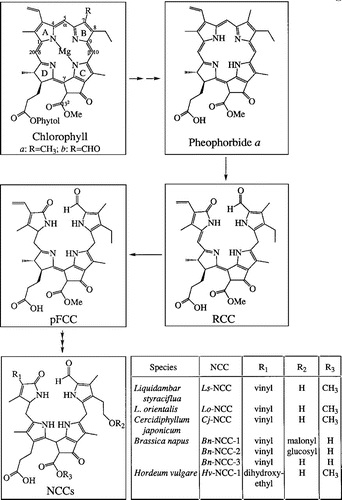
\includegraphics{figura1} \cite{Matile1999}\\
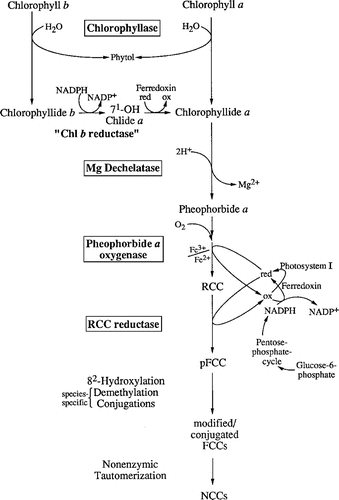
\includegraphics{figura2}



\end{document}